\documentclass{beamer}
\usepackage[utf8]{inputenc}
\usepackage[portuguese]{babel}
\usepackage{amsmath}
\usepackage{subfigure}
\usepackage{booktabs}
\usepackage{mhchem}             % chemical reactions
\usetheme{metropolis}           % Use metropolis theme

\newtheorem{mydefinition}{Definição}

\newcommand{\foreignword}[1]{\textit{#1}}
\newcommand{\toolname}[1]{\textit{#1}}
\newcommand{\fieldR}{\mathbb{R}}
\newcommand{\powerset}{\mathcal{P}}
\newcommand{\probability}{\mathbb{P}}
\newcommand{\expectation}{\mathbb{E}}
\newcommand{\algname}[1]{\texttt{#1}}
\newcommand{\langname}[1]{\texttt{#1}}
\newcommand{\varname}[1]{\texttt{#1}}
\newcommand{\floor}[1]{\lfloor #1 \rfloor}
\newcommand{\ceil}[1]{\lceil #1 \rceil}
\newcommand{\mathsc}[1]{{\normalfont\textsc{#1}}}
\newcommand{\species}[1]{\textit{#1}}
\newcommand{\gender}[1]{\textit{#1}}

\graphicspath{ {img/} }
\renewcommand*{\thesubfigure}{}

\title{Identification of cell signaling pathways based on biochemical 
reaction kinetics repositories}
\date{May 2019}
\author{Student: Gustavo Estrela\\
Advisor: Marcelo da Silva Reis (Butantan Institute)}
\institute{Instituto de Matemática e Estatística \\ 
           Centro de Toxinas, Resposta-imune e Sinalização Celular (CeTICS) \\
           Laboratório Especial de Ciclo Celular, Instituto Butantan\\
           \tiny{This project receives funding from FAPESP}}
\begin{document}

\maketitle
    
%Introduction
%- Cell Signaling Pathways;
%- Modeling it mathematically;
%- With a computational working computational model, we can enlight the
%  structure of a change of behaviour of a cell;
%- Creating a model;
    %- find a set of reactions;
    %- estimate the parameters of this model;
%- Lulu Wu created a method that systematically searches for a model, 
  %modifying it incrementally
    %- we can see the problem as a feature selection problem;
    %- it didn't work out so well...
    %- she was only able to reconstruct models if the starting model was
      %already similar to the correct model
    %- this may have happened because: the database could be more nearly
      %complete; the search algorithm could be more general; her cost 
      %function could not penalize well overcomplex functions.
%- We propose then to create a new methodology that overcomes theses 
  %difficulties using a new cost function, defining a broader search 
  %space and using new search algorithms.
%- Objectives of this work.



\begin{frame}{Cell Signaling}
Cell signaling allows cells to respond to signals that come from its 
environment changing its behaviour accordingly.
\pause

This mechanism is essential for many cell functions, including 
reproduction, growth and death.
\pause

Understanding the functioning of cell signaling is important in many 
biological areas.
\end{frame}


\begin{frame}{Cell Signaling}
\begin{figure}
    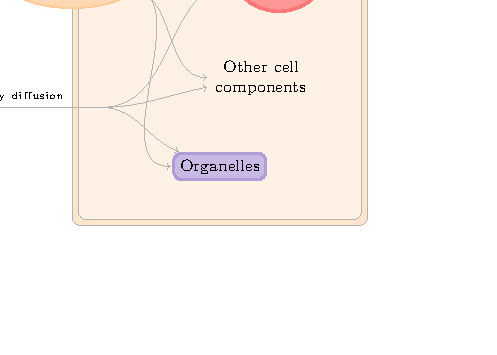
\includegraphics[clip=True, scale=.85]{introduction/signaling_mechanism.pdf}
\end{figure}
\end{frame}


\begin{frame}{Cell Signaling}
A signal propagates in an cell through chemical reactions that are
caused by the change of concentration of chemical species.

\pause
We call the path of a signal a cell signaling pathway.
\end{frame}


\begin{frame}{Cell Signaling Pathways}
A cell signaling network can be characterized by a sequence of chemical 
reactions 
\begin{figure}
    \includegraphics[scale=1.2, trim={.5cm 0 0 0}, clip]{introduction/csp_example.pdf}
\end{figure}
\end{frame}

\begin{frame}{Dynamic of Cell Signaling Pathways}
We can summarize the state of the cell signaling pathway with 
measurements based on the concentration of some chemical species.

\begin{figure}
    \includegraphics[scale=.3]{introduction/dynamic_example.png}
\end{figure}
\end{frame}


%fala sobre o output ser um modelo de equações diferenciais
%-> podemos mapear reações químicas em equações diferenciais
%-> com isso podemos simular o modelo e comparar com experimento

%Como achar esse modelo?
%-> precisamos determinar o conjunto de reações químicas da via
%-> precisamos achar suas constantes de velocidade
%...

%Lulu Wu resolveu este problema como um problema de seleção de 
%características... 


%O que propomos...

%Using biochemical and enzymatic kinetics, we can model the concentration
%change of chemical species over time of a pathway.



\begin{frame}{Identification of Cell Signaling Pathways}
The problem of identification of cell signaling pathways is the problem
of finding the components of a signaling pathway and how they interact
given a set of experimental measurement.

\pause
As the input, a description of a biological experiment and a set of 
experimental measurements are given. 
    
\pause A possible output to the problem is composed by:
\begin{itemize}
    \pause
    \item{a model composed by a set of chemical reactions that are 
        relevant for the biological experiment;}
    \pause
    \item{information about the reaction rate constants of the model.}
\end{itemize}
\end{frame}


\begin{frame}{A Model for Cell Signaling Pathways}
We model cell signaling pathways with a system of ordinary differential
equations. These equations represent the dynamic of concentrations of 
chemical species.
\end{frame}


\begin{frame}{Mathematical Models of Signaling Networks}
As an example, for the chemical reaction
\begin{equation*}
\ce{
    A + B -> C
},
\end{equation*}

\pause
we can write the following equation:
\begin{equation*}
    \frac{d[\text{C}]}{dt} = k[\text{A}][\text{B}]; 
\end{equation*}
where $k$ is a reaction rate constant.
\end{frame}



\begin{frame}{Identification of Cell Signaling Pathways}
How can one find which reactions are relevant for a given biological 
experiment? One can find good candidates by:
\pause
\begin{itemize}
    \item{using a priori information about the experiment;}
\pause
    \item{looking at biological databases such as KEGG.}
\end{itemize}
\pause
However, that might produce incomplete models, or models with 
unimportant reactions.

\pause
It is then desirable to systematically propose new models. 
\end{frame}


\begin{frame}{Identification of Cell Signaling Pathways}
Lulu Wu (2015) presented in her master dissertation a methodology that 
proposes to systematically modify models of signaling network in order
to better represent experiments.
\pause

On her work, the problem of identification of cell signaling pathways is
treated as a feature selection problem.
\end{frame}


\begin{frame}{Feature Selection Problem}
The feature selection problem can be defined in the following way:
\begin{center}
Given a set of features $S$ and a error function $err()$, find subset 
        $X \subseteq S$, with minimum error $err(X)$.
\end{center}
\end{frame}


\begin{frame}{Feature Selection for Identification of Signaling 
Pathways}
The methodology proposed by Wu defines the set of features as a set of 
chemical reactions that can be added to a starting model.\pause This set 
of chemical reactions is fetched from KEGG and stored in a database of
interactions.
\end{frame}


\begin{frame}{Dynamic of Cell Signaling Pathways}
\begin{flushleft}
\begin{figure}
    \includegraphics[scale=.57]{introduction/Lulu_methodology_diagram.pdf}
\end{figure}
\end{flushleft}
\end{frame}


\begin{frame}{Results of Wu's Methodology}
However, the methodology worked satisfactorily only when the Kernel 
model was similar to a correct model.
\end{frame}


\begin{frame}{Difficulties of Wu's Methodology}
We can point three aspects of Wu's work that could explain its 
limitations.
\begin{itemize}
\pause
\item{the database of interactions used could be more nearly complete;} 
\pause
\item{the search algorithm could also consider removing interactions;}
\pause
\item{the cost function could implement a proper penalization of 
models;}
\end{itemize}
\end{frame}


\begin{frame}{What we Propose on this Project}
We propose to create a methodology that uses a feature selection 
approach for identification of signaling pathways, tackling the 
difficulties encountered by Wu.
\end{frame}

\begin{frame}{What we Propose on this Project}
\begin{flushleft}
\begin{figure}
    \includegraphics[scale=.57]{introduction/my_dissertation_diagram.pdf}
\end{figure}
\end{flushleft}
\end{frame}


%\begin{frame}{What we Propose on this Project}
%To get a more nearly complete database of interactions, we should fetch 
%information from KEGG and other databases, \pause such as STRING and
%SABIO-RK.
%\end{frame}


%\begin{frame}{What we Propose on this Project}
%To use new search algorithms, \pause we intend to use more general
%algorithms that can also remove interactions.
%\end{frame}


%\begin{frame}{What we Propose on this Project}
%To define new cost functions, \pause we intend to use a Bayesian 
%approach of model selection that allow us to create estimates of 
%$p (D | M)$.
%\end{frame}


\begin{frame}{Objectives of this Project}
\begin{itemize}
\pause
\item{Build a database of interactions.}
\pause
\item{Create a cost function for models of signaling pathways.}
\pause
\item{Formulate systematic modifications to a model as the search space
    of a feature selection model.}
\pause
\item{Test the methodology on known signaling pathways and also on 
    pathways of interest in our lab.}
\end{itemize}
\end{frame}


\section{Bayesian Ranking of Models}
% To do the ranking we created SigNetMS
% - this software is able to create an estimate of the probability p (D | M)

% This probability is the marginal likelihood and to calculate that, we 
% also need to define p (D | M, \theta), which is the likelihood of 
% getting experimental data D in the context where M and \theta 
% represent the real model.
%
% - We assume this likelihood has a Gaussian distribution with mean zero
% and variance.
\begin{frame}{SigNetMS}
To perform model ranking, we created a Python package called SigNetMS.
\pause

Given a experimental data, a model and its constants priors, the 
software can calculate an estimative of $p (D | M)$. This value is 
called the marginal likelihood.
\end{frame}


\begin{frame}{SigNetMS}
SigNetMS is an open source software and it is available at:
\begin{center}
    \href{https://github.com/gustavoem/SigNetMS}{https://github.com/gustavoem/SigNetMS}
\end{center}
\end{frame}

\section{Experiments on Model Selection}
\begin{frame}{Model Ranking Experiment}
We tested SigNetMS on the ranking of models.
\end{frame}


\begin{frame}{Experiment description}
The experiment is based on the following procedure:
\begin{itemize}
    \pause
    \item{Create 4 candidate models.}
    \pause
    \item{For one of the models, choose a set of parameter values 
        and time steps and simulate data.}
    \pause
    \item{Add Gaussian noise to the simulations. Repeat two more 
        times to generate three observations of the system.}
    \pause
    \item{Neglect chosen parameter values and define prior distributions
        for every parameter.}
    \pause
    \item{Rank the four models.}
\end{itemize}
\end{frame}


\begin{frame}{Model Ranking Experiment}
\begin{figure}
  \begin{tabular}{c c}
    \subfigure[Model 1]{
    \includegraphics[clip=true,width=.42\linewidth]{experiments/diagrams/bioinformatics_model1.pdf}}
    &
    \subfigure[Model 2]{
    \includegraphics[clip=true,width=.42\linewidth]{experiments/diagrams/bioinformatics_model2.pdf}}
    \\
    \subfigure[Model 3] {
    \includegraphics[clip=true,width=.42\linewidth]{experiments/diagrams/bioinformatics_model3.pdf}}
    &
    \subfigure[Model 4] {
    \includegraphics[clip=true,width=.42\linewidth]{experiments/diagrams/bioinformatics_model4.pdf}}
    \end{tabular}
\end{figure}
\end{frame}


\begin{frame}{Results on SigNetMS}
The ranking returned by SigNetMS on the experiment is:
\begin{equation*}
    1 > 2 > 4 > 3;
\end{equation*}

\pause
Note that:
\pause
\begin{itemize}
    \item{the correct model is ranked first;}
    \item{overly complex models are ranked worse than simpler models.}
\end{itemize}
\end{frame}

\begin{frame}{Results on SigNetMS}
\vspace{-2em}
\begin{figure}
    \centering
    \begin{tabular}{c c}
    \subfigure{
    \includegraphics[clip=true,width=.46\linewidth]{experiments/results/girolami/gamma/snm/simulations_model1_39.png}}
    &
    \subfigure{
    \includegraphics[clip=true,width=.46\linewidth]{experiments/results/girolami/gamma/snm/simulations_model2_39.png}} 
    \\
    \subfigure{
    \includegraphics[clip=true,width=.46\linewidth]{experiments/results/girolami/gamma/snm/simulations_model3_39.png}} 
    &
    \subfigure{
    \includegraphics[clip=true,width=.46\linewidth]{experiments/results/girolami/gamma/snm/simulations_model4_39.png}} 
    \end{tabular}
\end{figure}
\end{frame}


\begin{frame}{Surface Walk Experiment}
We also designed an experiment to walk on search space of models. The
experiment consists in starting with a base model and then iteratively 
add reactions to it randomly, calculating their scores. 

\pause
The scores are calculated in respect to experimental data generated by
a model that is present in the search space.
\end{frame}


\begin{frame}{Surface Walk Experiment}
\begin{figure}
    \includegraphics[scale=1.2]{experiments/surface_walk/correct_model.pdf}
\end{figure}
\end{frame}

\begin{frame}{Surface Walk Experiment}
\begin{figure}
    \includegraphics[scale=1.2]{experiments/surface_walk/base_model.pdf}
\end{figure}
\end{frame}

\begin{frame}{Surface Walk Experiment}
\begin{figure}
    \includegraphics[scale=0.6]{experiments/surface_walk/surface_curve.png}
\end{figure}
\end{frame}

\section{Future Work}

\begin{frame}{Future Work}
More activities are expected to be completed in this project, mainly the
follow:
\begin{itemize}
    %\item{} Embedding SigNetMS as a cost function for featsel, a 
        %framework for feature selection.
    %\pause
    \item{} Creation of a relational database of chemical 
        interactions focused on our further applications.
    \end{itemize}
\end{frame}


\begin{frame}{Future Work}
\begin{itemize}
    %\item{} Choice of a feature selection search algorithm.
    %\pause
    \item{} Apply the method in ERK signaling 
        pathways of tumor cell lines Y1 and HEK293.
\end{itemize}
\end{frame}

\begin{frame}{}
\begin{center}
    \texttt{Thank you!}
\end{center}
\end{frame}

\end{document}
